\nonstopmode

\documentclass[11pt]{article}

\usepackage{amsmath}
\usepackage[utf8]{inputenc}
\usepackage{graphicx}

\usepackage{siunitx}
\usepackage{tikz} % To generate the plot from csv
\usepackage{pgfplots}

\pgfplotsset{compat=newest} % Allows to place the legend below plot
\usepgfplotslibrary{units} % Allows to enter the units nicely

\sisetup{
  round-mode          = places,
  round-precision     = 2,
}

\title{Software Development Principles}
\author{Phoomparin Mano}
\date{May 2019}

\begin{document}
  \maketitle

  \section{Introduction}

  \subsection{Huh}

  Alright. Let's begin with an equation:

  \begin{equation}
    f(x) = x^2 e ^2 - \frac{5}{8} \lambda
  \end{equation}
  
  \begin{equation*}
  	\lambda 5 \lambda 3
  \end{equation*}

  Also, here's another equation.

  \subsection{Woah}

  \section{Hello World!}

  \begin{equation}
    f(g(x)) = g(f(x))
  \end{equation}

  \begin{equation*}
    \lambda a \cdot b \cdot ab
  \end{equation*}

  Welcome, \[f(g(x)) = g(f(x))\].

  \begin{align*}
    1 + 2 &= 3 \\
    1 &= 3 - 6
  \end{align*}

  \begin{equation*}
    \int^a_b \frac{1}{3} x^3

    \left[
      \begin{matrix}
        1 & 0\\
        0 & 1
      \end{matrix}
    \right]
  \end{equation*}

  \section{What is going on dafuq!}

  \begin{figure}[h!]
    \begin{center}
      \begin{tikzpicture}
        \begin{axis}[
            width=\linewidth, % Scale the plot to \linewidth
            grid=major, % Display a grid
            grid style={dashed,gray!30}, % Set the style
            xlabel=X Axis $U$, % Set the labels
            ylabel=Y Axis $I$,
            x unit=\si{\volt}, % Set the respective units
            y unit=\si{\ampere},
            legend style={at={(0.5,-0.2)},anchor=north}, % Put the legend below the plot
            x tick label style={rotate=90,anchor=east} % Display labels sideways
          ]
          \addplot+ [
            color = purple,
            mark options={
              color = purple,
              draw = purple,
              fill = purple
            }
          ]
          % add a plot from table; you select the columns by using the actual name in
          % the .csv file (on top)
          table[x=time,y=space,col sep=comma] {table.csv};
          \legend{Plot}
        \end{axis}
      \end{tikzpicture}
      \caption{My first autogenerated plot.}
    \end{center}
  \end{figure}

  \section{Plotting}

  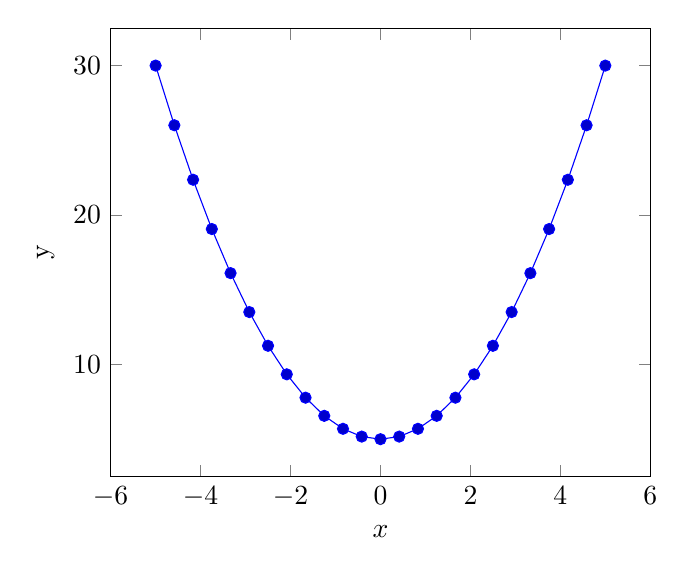
\begin{tikzpicture}
    \begin{axis}[
      xlabel=$x$,
      ylabel={y}
    ]

    \addplot {x ^ 2 + 5};
    \end{axis}
  \end{tikzpicture}

  \section{Lambda}

  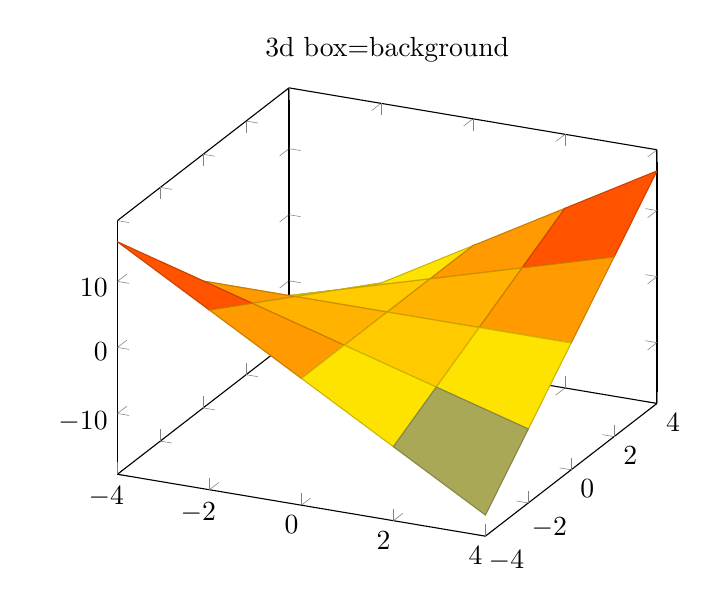
\begin{tikzpicture}
    \begin{axis}[
      3d box=background,
      % pretty printing, but irrelevant:
      title={3d box=background},
      samples=5,
      domain=-4:4,
      xtick=data,
      ytick=data,
    ]
      \addplot3[surf] {x*y};
    \end{axis}
  \end{tikzpicture}
\end{document}

